\hypertarget{group__xEventGroupSync}{}\section{x\+Event\+Group\+Sync}
\label{group__xEventGroupSync}\index{x\+Event\+Group\+Sync@{x\+Event\+Group\+Sync}}
Collaboration diagram for x\+Event\+Group\+Sync\+:\nopagebreak
\begin{figure}[H]
\begin{center}
\leavevmode
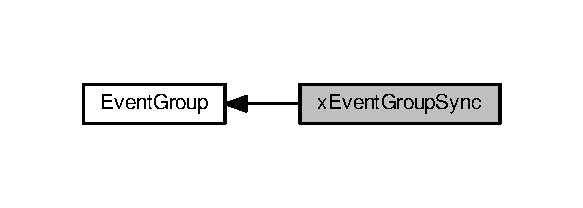
\includegraphics[width=280pt]{d2/dd3/group__xEventGroupSync}
\end{center}
\end{figure}
\hyperlink{event__groups_8h}{event\+\_\+groups.\+h} 
\begin{DoxyPre}
   EventBits\_t xEventGroupSync( EventGroupHandle\_t xEventGroup,
                                const EventBits\_t uxBitsToSet,
                                const EventBits\_t uxBitsToWaitFor,
                                TickType\_t xTicksToWait );
\end{DoxyPre}


Atomically set bits within an event group, then wait for a combination of bits to be set within the same event group. This functionality is typically used to synchronise multiple tasks, where each task has to wait for the other tasks to reach a synchronisation point before proceeding.

This function cannot be used from an interrupt.

The function will return before its block time expires if the bits specified by the ux\+Bits\+To\+Wait parameter are set, or become set within that time. In this case all the bits specified by ux\+Bits\+To\+Wait will be automatically cleared before the function returns.


\begin{DoxyParams}{Parameters}
{\em x\+Event\+Group} & The event group in which the bits are being tested. The event group must have previously been created using a call to x\+Event\+Group\+Create().\\
\hline
{\em ux\+Bits\+To\+Set} & The bits to set in the event group before determining if, and possibly waiting for, all the bits specified by the ux\+Bits\+To\+Wait parameter are set.\\
\hline
{\em ux\+Bits\+To\+Wait\+For} & A bitwise value that indicates the bit or bits to test inside the event group. For example, to wait for bit 0 and bit 2 set ux\+Bits\+To\+Wait\+For to 0x05. To wait for bits 0 and bit 1 and bit 2 set ux\+Bits\+To\+Wait\+For to 0x07. Etc.\\
\hline
{\em x\+Ticks\+To\+Wait} & The maximum amount of time (specified in \textquotesingle{}ticks\textquotesingle{}) to wait for all of the bits specified by ux\+Bits\+To\+Wait\+For to become set.\\
\hline
\end{DoxyParams}
\begin{DoxyReturn}{Returns}
The value of the event group at the time either the bits being waited for became set, or the block time expired. Test the return value to know which bits were set. If \hyperlink{event__groups_8h_a869511456b86426f52e2eec898bff341}{x\+Event\+Group\+Sync()} returned because its timeout expired then not all the bits being waited for will be set. If \hyperlink{event__groups_8h_a869511456b86426f52e2eec898bff341}{x\+Event\+Group\+Sync()} returned because all the bits it was waiting for were set then the returned value is the event group value before any bits were automatically cleared.
\end{DoxyReturn}
Example usage\+: 
\begin{DoxyPre}
// Bits used by the three tasks.
#define TASK\_0\_BIT      ( 1 << 0 )
#define TASK\_1\_BIT      ( 1 << 1 )
#define TASK\_2\_BIT      ( 1 << 2 )\end{DoxyPre}



\begin{DoxyPre}#define ALL\_SYNC\_BITS ( TASK\_0\_BIT | TASK\_1\_BIT | TASK\_2\_BIT )\end{DoxyPre}



\begin{DoxyPre}// Use an event group to synchronise three tasks.  It is assumed this event
// group has already been created elsewhere.
EventGroupHandle\_t xEventBits;\end{DoxyPre}



\begin{DoxyPre}void vTask0( void *pvParameters )
\{
EventBits\_t uxReturn;
TickType\_t xTicksToWait = 100 / portTICK\_PERIOD\_MS;
\begin{DoxyVerb}for( ;; )
{
// Perform task functionality here.

// Set bit 0 in the event flag to note this task has reached the
// sync point.  The other two tasks will set the other two bits defined
// by ALL_SYNC_BITS.  All three tasks have reached the synchronisation
// point when all the ALL_SYNC_BITS are set.  Wait a maximum of 100ms
// for this to happen.
uxReturn = xEventGroupSync( xEventBits, TASK_0_BIT, ALL_SYNC_BITS, xTicksToWait );

if( ( uxReturn & ALL_SYNC_BITS ) == ALL_SYNC_BITS )
{
    // All three tasks reached the synchronisation point before the call
    // to xEventGroupSync() timed out.
}
\end{DoxyVerb}

   \}
\}\end{DoxyPre}



\begin{DoxyPre}void vTask1( void *pvParameters )
\{
    for( ;; )
    \{
    // Perform task functionality here.\end{DoxyPre}



\begin{DoxyPre}    // Set bit 1 in the event flag to note this task has reached the
    // synchronisation point.  The other two tasks will set the other two
    // bits defined by ALL\_SYNC\_BITS.  All three tasks have reached the
    // synchronisation point when all the ALL\_SYNC\_BITS are set.  Wait
    // indefinitely for this to happen.
    xEventGroupSync( xEventBits, TASK\_1\_BIT, ALL\_SYNC\_BITS, portMAX\_DELAY );\end{DoxyPre}



\begin{DoxyPre}    // \hyperlink{event__groups_8h_a869511456b86426f52e2eec898bff341}{xEventGroupSync()} was called with an indefinite block time, so
    // this task will only reach here if the syncrhonisation was made by all
    // three tasks, so there is no need to test the return value.
    \}
\}\end{DoxyPre}



\begin{DoxyPre}void vTask2( void *pvParameters )
\{
    for( ;; )
    \{
    // Perform task functionality here.\end{DoxyPre}



\begin{DoxyPre}    // Set bit 2 in the event flag to note this task has reached the
    // synchronisation point.  The other two tasks will set the other two
    // bits defined by ALL\_SYNC\_BITS.  All three tasks have reached the
    // synchronisation point when all the ALL\_SYNC\_BITS are set.  Wait
    // indefinitely for this to happen.
    xEventGroupSync( xEventBits, TASK\_2\_BIT, ALL\_SYNC\_BITS, portMAX\_DELAY );\end{DoxyPre}



\begin{DoxyPre}    // \hyperlink{event__groups_8h_a869511456b86426f52e2eec898bff341}{xEventGroupSync()} was called with an indefinite block time, so
    // this task will only reach here if the syncrhonisation was made by all
    // three tasks, so there is no need to test the return value.
   \}
\}\end{DoxyPre}



\begin{DoxyPre}\end{DoxyPre}
 